\documentclass[11pt,a4paper,parskip=half]{scrartcl}
\usepackage{isabelle,isabellesym}

% further packages required for unusual symbols (see also
% isabellesym.sty), use only when needed

%\usepackage{amssymb}
  %for \<leadsto>, \<box>, \<diamond>, \<sqsupset>, \<mho>, \<Join>,
  %\<lhd>, \<lesssim>, \<greatersim>, \<lessapprox>, \<greaterapprox>,
  %\<triangleq>, \<yen>, \<lozenge>

%\usepackage[greek,english]{babel}
  %option greek for \<euro>
  %option english (default language) for \<guillemotleft>, \<guillemotright>

\usepackage[only,bigsqcap]{stmaryrd}
  %for \<Sqinter>

%\usepackage{eufrak}
  %for \<AA> ... \<ZZ>, \<aa> ... \<zz> (also included in amssymb)

%\usepackagetcomp}
  %for \<onequarter>, \<onehalf>, \<threequarters>, \<degree>, \<cent>,
  %\<currency>

% for uniform font size
%\renewcommand{\isastyle}{\isastyleminor}

% From src/HOL/HOLCF/document/root
\newcommand{\isasymnotsqsubseteq}{\isamath{\not\sqsubseteq}}

\usepackage{amsmath}
\usepackage{amsfonts}
\usepackage{mathtools}
\usepackage{graphicx}
\usepackage{tikz}
\usepackage[T1]{fontenc}
\usepackage[utf8]{inputenc}
\usepackage{mathpartir}
\usepackage{calc}

\usepackage{floatpag}
\floatpagestyle{empty}

% this should be the last package used
\usepackage{pdfsetup}

% silence the KOMA script warnings
\def\bf{\normalfont\bfseries}
\def\it{\normalfont\itshape}
\def\rm{\normalfont\rmfamily}


% urls in roman style, theorys in math-similar italics
\urlstyle{rm}
\isabellestyle{it}

% Isabelle does not like *} in a text {* ... *} block
% Concrete implemenation thanks to http://www.mrunix.de/forums/showpost.php?p=235085&postcount=5
\newenvironment{alignstar}{\csname align*\endcsname}{\csname endalign*\endcsname}
\newenvironment{alignatstar}{\csname alignat*\endcsname}{\csname endalignat*\endcsname}


% Entering \ in Isabelle/jEdit has unwanted consequences
\catcode`\|=0 %

\begin{document}

\title{The Correctness and Adequacy of Launchbury's Natural Semantics for Lazy Evaluation}
\author{Joachim Breitner\\
Programming Paradigms Group\\
Karlsruhe Institute for Technology\\
\url{breitner@kit.edu}}
\maketitle

\begin{abstract}
In his seminal paper „Natural Semantics for Lazy Evaluation“ \cite{launchbury},
John Launchbury proves his semantics correct with respect to a denotational
semantics, and outlines an adequacy proof.
We have formalized both semantics and machine-checked the correctness proof,
clarifying some details.
Furthermore, we provide a new and more direct adequacy proof that does not
require intermediate operational semantics.
\end{abstract}

\tableofcontents

\section{Introduction}

The Natural Semantics for Lazy Evaluation \cite{launchbury} created by John Launchbury in 1992 is often taken as the base for formal treatments of call-by-need evaluation, either to prove properties of lazy evaluation or as a base to describe extensions of the language or the implementation of the language. Therefore, assurance about the correctness and adequacy of the semantics is important in this field of research. Launchbury himself supports his semantics by defining a standard denotational semantics to prove both correctness and adequacy.

Although his proofs are already on the more rigorous side for pen-and-paper proofs, they have not yet been verified by transforming them to machine-checked proofs.
The present work fills this gap by formalizing both semantics in the proof assistant Isabelle and proving both correctness and adequacy.

Our correctness formal proof is very close to the original proof. This is possible if the operator $\sqcup$ is understood as a right-sided update. If we were to understand $\sqcup$ as the least upper bound, then Theorem 2 in \cite{launchbury}, which is the generalization of the correctness statement used for Launchbury's inductive proof, is wrong. The main correctness result still holds, but needs a different proof; this is discussed in greater detail in \cite{breitner2013}.

Launchbury outlines an adequacy proof via an intermediate operational semantics and resourced denotational semantics. The alternative operational semantics  uses indirection instead of substitution for applications, does not update variable results and does not perform blackholing during evaluation of a variable. The equivalence of these two operational semantics is hard and tricky to prove. We found a direct proof for the adequacy of the original operational semantics and the (slightly modified) resourced denotational semantics. This is, as far as we know, the first complete and rigorous proof of adequacy of Launchbury's semantics.

Our contributions are:
\begin{itemize}
\item We define the natural and denotational semantics given by Launchbury in the theorem prover Isabelle.
\item We demonstrate how to use both the Nominal package (to handle name binding) \cite{nominal} and the HOLCF \cite{holcf} package (for the domain-theoretic aspects) in the same development.
\item We verify Launchbury's proof of correctness.
\item We provide a new and more direct proof of adequacy.
\item In order to do so, we formalize parts of \cite{functionspaces}, fixing a mistake in the proof.
\end{itemize}

%\subsubsection{The big picture}

The following picture gives an overview of the different semantics. Elements printed in black are formally defined and proved in the present work, while the gray square on the left shows the proofs and propositions in Launchbury’s original work \cite{launchbury}.

\begin{center}
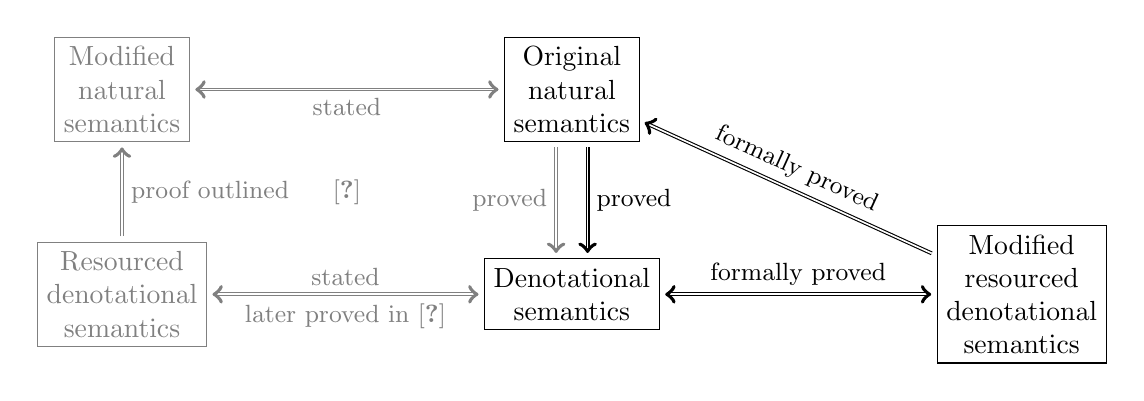
\begin{tikzpicture}[every node/.style={align=center}]
\matrix (m) [row sep=3em, column sep=10em] 
{ \node[draw,gray] (mn) {Modified\\natural\\semantics}; & \node[draw] (on) {Original\\natural\\semantics}; &; \\
  \node[draw,gray] (rd) {Resourced\\denotational\\semantics}; & \node[draw] (jd) {Denotational\\semantics}; & \node[draw] (sn) {Modified\\resourced\\denotational\\semantics} ;
  %\node[draw] (ud) {Denotational\\semantics\\with update};
  \\
};

\small
\draw[gray,<->,double, shorten <=.5ex, shorten >= .5ex]  (on) -- (mn) node[midway,below] {stated};
\draw[gray,->,double, shorten <=.5ex, shorten >= .5ex]  (rd) -- (mn) node[midway,right] {proof outlined};
\draw[gray,<->,double, shorten <=.5ex, shorten >= .5ex]  (rd) -- (jd) node[midway,above] {stated} 
                                                            node[midway,below] {later proved in \cite{functionspaces}};
\draw[transform canvas={xshift=2mm},->,double, shorten <=.5ex, shorten >= .5ex] (on) -- (jd) node[midway,right] {proved};
\draw[transform canvas={xshift=-2mm},gray,->,double, shorten <=.5ex, shorten >= .5ex] (on) -- (jd) node[midway,left] {proved};
\draw[<-,double, shorten <=.5ex, shorten >= .5ex]  (on) -- (sn) node[sloped,midway,above] {formally proved};
\draw[<->,double, shorten <=.5ex, shorten >= .5ex] (sn) -- (jd.east) node[sloped,midway,above] {formally proved};
%\draw[->,double, shorten <=.5ex, shorten >= .5ex] (on) -- (ud) node[sloped,midway,above] {Proof};
%\draw[<->,double, shorten <=.5ex, shorten >= .5ex]  (jd) -- (ud) node[midway,below] {formally proved};
\node[gray] at (barycentric cs:on=1,mn=1,rd=1,jd=1) {\cite{launchbury}};
\end{tikzpicture}
\end{center}


\input{EverythingAdequacy.tex}


\begin{figure}
\begin{center}
\IfFileExists{session_graph.pdf}{
  \includegraphics[width=\textwidth]{session_graph}
}{Here, \texttt{session\_graph.pdf} would be shown.}
\end{center}
\caption{Theory Dependency Graph\label{theory-deps}}
\end{figure}

\subsection{Theory overview}

The following chapters contain the complete Isabelle theories, with one section per theory. Their interdependencies are visualized in Figure \ref{theory-deps}.

Chapter \ref{ch_aux} contains auxiliary theories, not necessarily tied to Launchbury's semantics. The base theories are kept independent of Nominal and HOLCF where possible, the lemmas combining them are in theories of their own, creatively named by appending \isa{-Nominal} resp.\ \isa{-HOLCF}.  You will find these theories:
\begin{itemize}
\item A definition for lifting a relation point-wise (\isa{Pointwise}).
\item A collection of definition related to associative lists (\isa{AList-Utils}, \isa{AList-Utils-Nominal}).
\item A characterization of monotonous functions $\mathbb N \to \mathbb N$ (\isa{Mono-Nat-Fun}).
\item General utility functions extending Nominal (\isa{Nominal-Utils}).
\item General utility functions extending HOLCF (\isa{HOLCF-Utils}).
\item Binary meets in the context of HOLCF (\isa{HOLCF-Meet}).
\item A theory combining notions from HOLCF and Nominal, e.g.\ continuity of permutation (\isa{Nominal-HOLCF}).
\item A theory for working with pcpo-valued functions as semantic environments (\isa{Env}, \isa{Env-Nominal}, \isa{Env-HOLCF}).
\item A function \isa{evalHeap} that converts between associative lists and functions. (\isa{EvalHeap})
\end{itemize}

Chapter \ref{ch_natsem} defines the syntax and Launchbury's natural semantics.

Chapter \ref{ch_dendom} sets the stage for the denotational semantics by defining a locale \isa{semantic-domain} for denotational domains, and an instantiation for the standard domain.

Chapter \ref{ch_den} defines the denotational semantics. It also introduces the locale \isa{has-ESem} which abstracts over the value semantics when defining the semantics of heaps.

Chapter \ref{ch_resden} defines the resourced denotational semantics.

Chapter \ref{ch_correctness} proves the correctness of Launchbury's semantics with regard to both denotational semantics. We need the correctness with regard to the resourced semantics in the adequacy proof.

Chapter \ref{ch_equiv} proves the two denotational semantics related, which is used in

Chapter \ref{ch_adequacy}, where finally the adequacy is proved.

%\subsection{Reusable components}
%
%Parts of this theory are independent of the actual semantics and may be of use to other users of Isabelle:
%
%TODO

\subsection{Acknowledgements}

%I’d like to thank Andreas Lochbihler for his gladly given and very effective help during the development of this theory. I’d also like to thank Brian Huffmann and Christian Urban for their help on HOLCF and Nominal, respectively. This work was supported by the Deutsche Telekom Stiftung.

I’d like to thank Lidia Sánchez-Gil, Mercedes Hidalgo-Herrero and Yolanda Ortega-Mallén for inviting me to Madrid to discuss our respective approaches.\\
This work was supported by the Deutsche Telekom Stiftung.

\clearpage
\newcommand{\theory}[1]{\subsection{#1}\label{sec_#1}\input{#1.tex}}

\section{Auxillary theories}
\label{ch_aux}

\theory{Pointwise}
\theory{AList-Utils}
\theory{Mono-Nat-Fun}

\theory{Nominal-Utils}
\theory{AList-Utils-Nominal}

\theory{HOLCF-Utils}
\theory{HOLCF-Meet}
\theory{Nominal-HOLCF}


\theory{Env}
\theory{Env-Nominal}
\theory{Env-HOLCF}
\theory{EvalHeap}


\clearpage
\section{Launchbury's natural semantics}
\label{ch_natsem}

\theory{Vars}
\theory{Terms}
\theory{Substitution}
\theory{Launchbury}

\section{Denotational domain}
\label{ch_dendom}

\theory{Value}
\theory{Value-Nominal}


\clearpage
\section{Denotational semantics}
\label{ch_den}

\theory{Iterative}
\theory{HasESem}
\theory{HeapSemantics}
\theory{AbstractDenotational}
\theory{Abstract-Denotational-Props}
\theory{Denotational}


\clearpage
\section{Resourced denotational domain}
\label{ch_resden}

\theory{C}
\theory{C-Meet}
\theory{C-restr}
\theory{CValue}
\theory{CValue-Nominal}
\theory{ResourcedDenotational}


\clearpage
\section{Correctness of the natural semantics}
\label{ch_correctness}

\theory{CorrectnessOriginal}
\theory{CorrectnessResourced}

\clearpage
\section{Equivalence of the denotational semantics}
\label{ch_equiv}

\theory{ValueSimilarity}
\theory{Denotational-Related}

\clearpage
\section{Adequacy}
\label{ch_adequacy}

\theory{ResourcedAdequacy}
\theory{Adequacy}


%\clearpage
%\section{Conclusion}
%
%TODO

\clearpage
\bibliographystyle{amsalpha}
\bibliography{root_adequacy}

\end{document}
